% Two points p, q of a Hausdorff space separated by disjoint open
% neighborhoods (dashed disks).
% Source: book/tex/topology/top-more.tex (§ Hausdorff spaces).
\documentclass[border=2mm]{standalone}
\usepackage{tikz}
\begin{document}
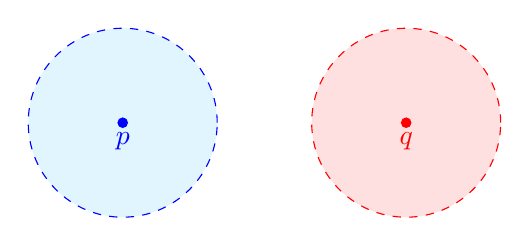
\begin{tikzpicture}[scale=1.2]
  \fill[cyan!12] (-1.5,0) circle (1);
  \draw[blue, dashed] (-1.5,0) circle (1);
  \fill[red!12] (1.5,0) circle (1);
  \draw[red, dashed] (1.5,0) circle (1);
  \fill[blue] (-1.5,0) circle (1.6pt) node[below, blue] {$p$};
  \fill[red] (1.5,0) circle (1.6pt) node[below, red] {$q$};
\end{tikzpicture}
\end{document}
